% Please use the skeleton file you have received in the
% invitation-to-submit email, where your data are already
% filled in. Otherwise please make sure you insert your
% data according to the instructions in PoSauthmanual.pdf
\documentclass{PoS}

\title{Search for SUSY with a customized top tagger with the CMS experiment}

\ShortTitle{Short Title for header}

\author
{
  %\speaker{Hua Wei}\thanks{A footnote may follow.}\\
  \speaker{Hua Wei}\\
  CMS collabration\\
  University of California, Riverside\\
  E-mail: \email{hua.wei@cern.ch}
}

%\author{Another Author\\
%        Affiliation\\
%        E-mail: \email{...}}

\abstract{This proceeding presents a search for direct and gluino-mediated production of supersymmetric scalar top-quark pairs in the all-hadronic final state using top tagging. The result of search is based on a 13 TeV proton-proton sample collected with the CMS detector at the LHC in 2016, corresponding to an integrated luminosity of $36~fb^{-1}$. The results of the search are interpreted in several Simplified Models (SMS).}

\FullConference
{
  EPS-HEP 2017, European Physical Society conference on High Energy Physics\\
  5-12 July 2017\\
  Venice, Italy
}

\begin{document}

\section{Introduction}

The supersymmetric extension of the standard model is a promising solution for the hierarchy problem in the standard model. can be cured with the existence of light higgsino, top squarks, bottom squark or gluino, which can decay into lightest supersymmetric particle (LSP). The LSP can be neutral and stable under R-parity conservation, which provide us a candidate for dark matter. Therefore, supersymmetry represents an exciting theory for us to explore.

A search in missing transverse energy, extended transverse mass, b-jets and top-quarks final state are presented in this proceeding. A customized top-jet tagging algorithm was designed in order to obtain the relatively high efficiency for all relevant values of the top quark transverse momentum.

\section{Top Tagger}
\section{Results}

The analysis interpretations are presented in Fig~\ref{fig:signal_results}. 

\begin{figure}[ht!]
 \begin{centering}
  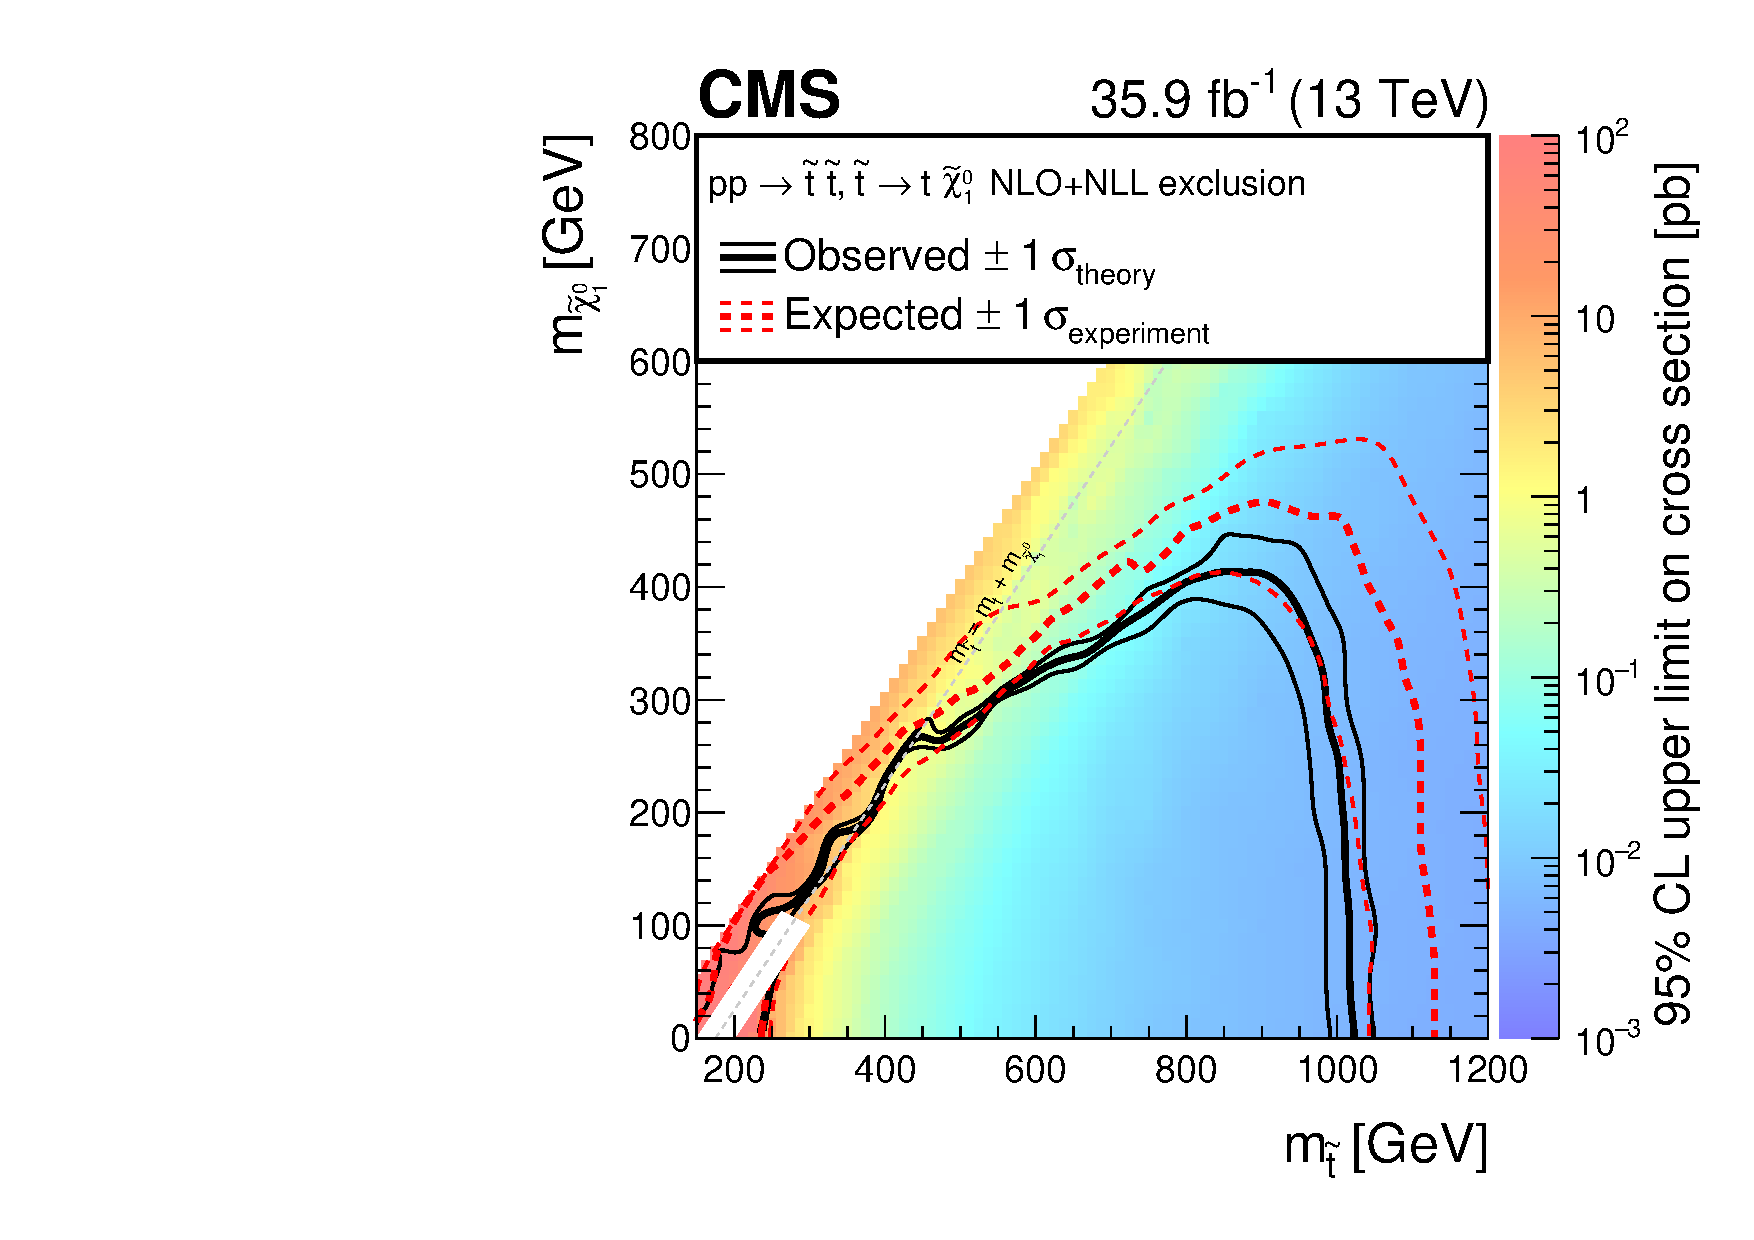
\includegraphics[width=0.40\textwidth]{figures/Covered_T2tt_OnlyXSEC.pdf}
  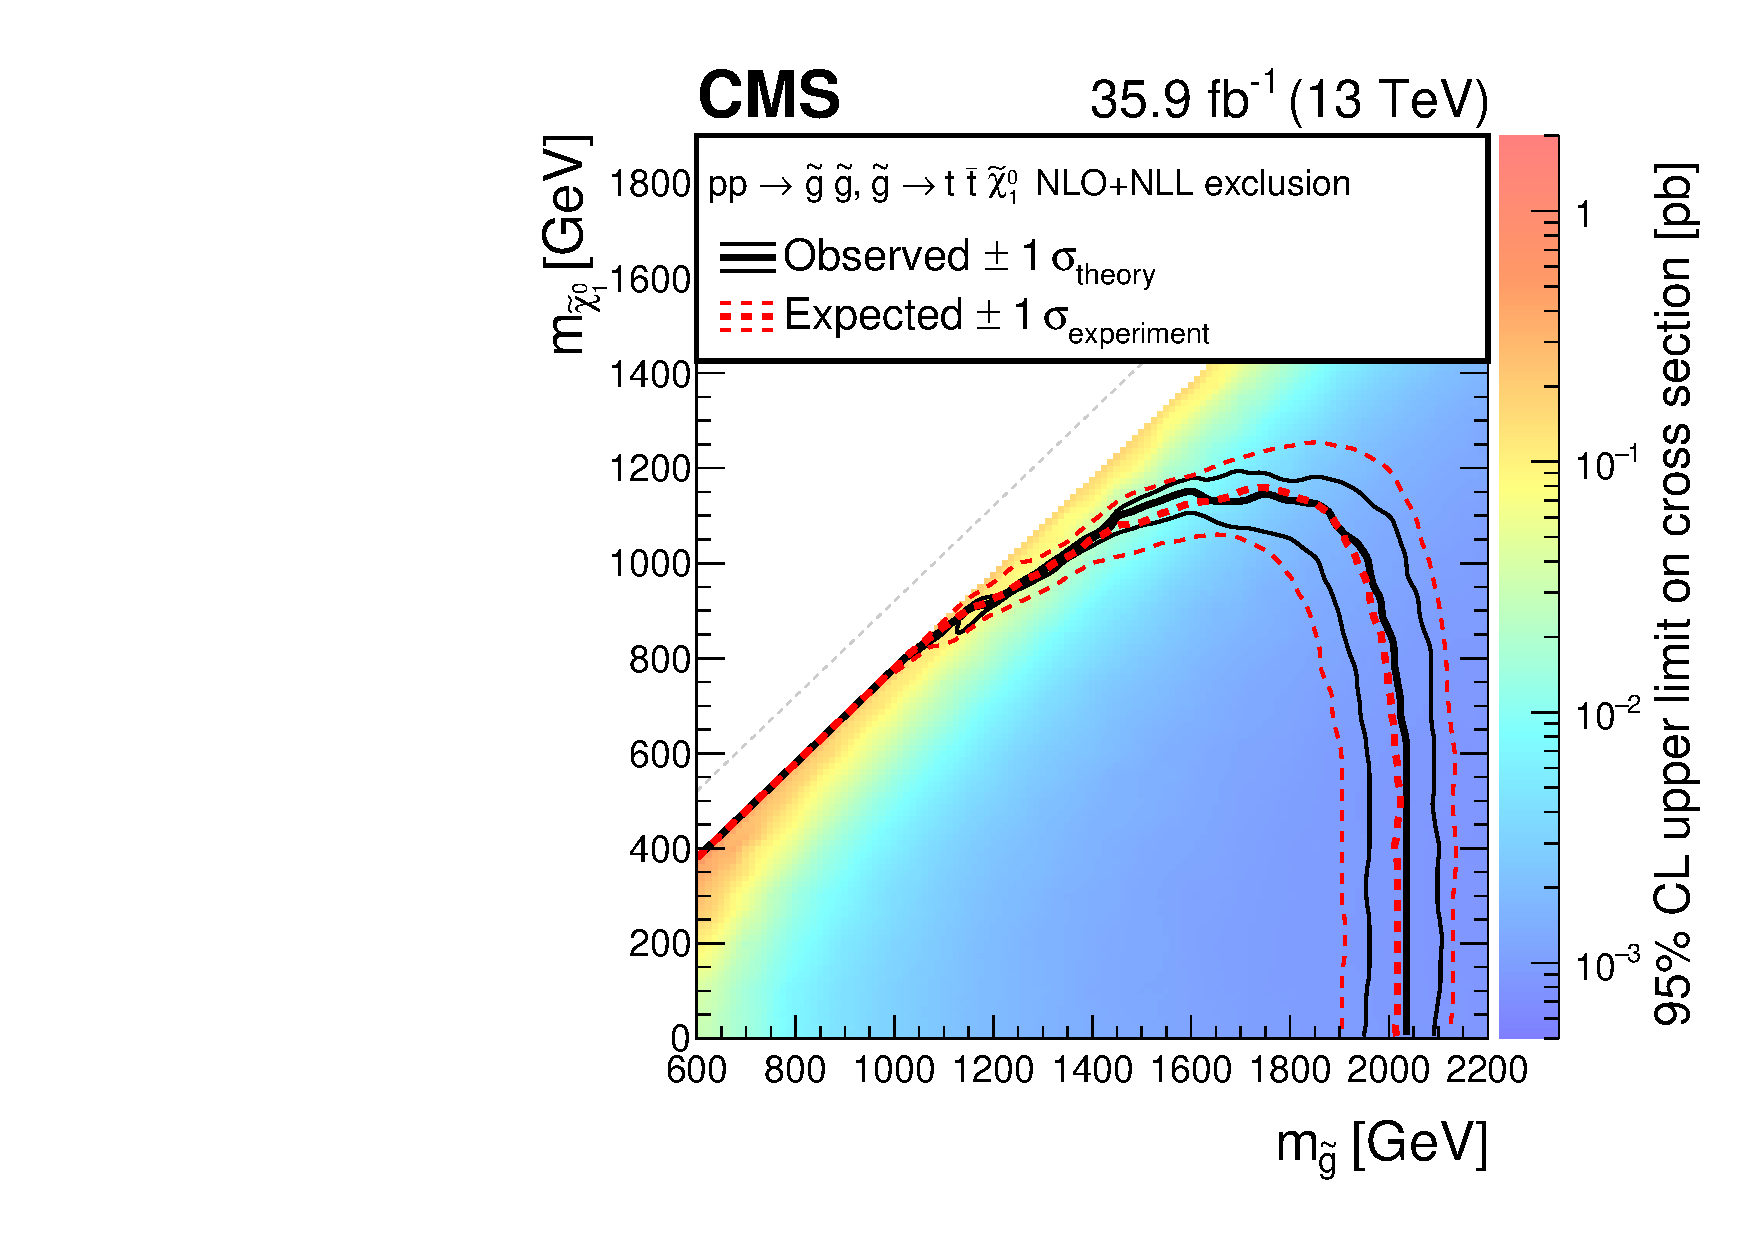
\includegraphics[width=0.40\textwidth]{figures/T1tttt_OnlyXSEC.pdf}
  \caption{Exclusion limit at 95\% CL for the signal models in this search: top squark pair production with the top squark decaying into a top quark and neutralino (T2tt, left), and top squarks from cascade decays of gluinos (T1tttt, right).}
  \label{fig:signal_results}
 \end{centering}
\end{figure}

No excess of events above the expected standard model background is observed. The result is interpreted in the context of simplified supersymmetric models as 95\% confidence level upper limits on the cross section of gluinos and top squarks pair production processes. The T2tt model has been excluded for top squark masses up to 1020 GeV. The corresponding exclusions on the gluino mass are up to 1810-2040 GeV, depending on the type of models. The naturalness\cite{Papucci:2011wy} of the SUSY MSSM RPC simplified models are under challenge with large 13 TeV data samples now being collected at the LHC.

%\begin{thebibliography}{99}
%\bibitem{latexcompanion} 
%Michel Goossens, Frank Mittelbach, and Alexander Samarin. 
%\textit{The \LaTeX\ Companion}. 
%Addison-Wesley, Reading, Massachusetts, 1993.
%\end{thebibliography}
\bibliographystyle{JHEP}
\bibliography{refproceeding}

\end{document}
